
\documentclass[a4paper,12pt]{article}
%%%%%%%%%%%%%%%%%%%%%%%%%%%%%%%%%%%%%%%%%%%%%%%%%%%%%%%%%%%%%%%%%%%%%%%%%%%%%%%%%%%%%%%%%%%%%%%%%%%%%%%%%%%%%%%%%%%%%%%%%%%%%%%%%%%%%%%%%%%%%%%%%%%%%%%%%%%%%%%%%%%%%%%%%%%%%%%%%%%%%%%%%%%%%%%%%%%%%%%%%%%%%%%%%%%%%%%%%%%%%%%%%%%%%%%%%%%%%%%%%%%%%%%%%%%%
\usepackage{eurosym}
\usepackage{vmargin}
\usepackage{amsmath}
\usepackage{graphics}
\usepackage{epsfig}
\usepackage{framed}
\usepackage{subfigure}
\usepackage{fancyhdr}

\setcounter{MaxMatrixCols}{10}
%TCIDATA{OutputFilter=LATEX.DLL}
%TCIDATA{Version=5.00.0.2570}
%TCIDATA{<META NAME="SaveForMode"CONTENT="1">}
%TCIDATA{LastRevised=Wednesday, February 23, 201113:24:34}
%TCIDATA{<META NAME="GraphicsSave" CONTENT="32">}
%TCIDATA{Language=American English}

\pagestyle{fancy}
\setmarginsrb{20mm}{0mm}{20mm}{25mm}{12mm}{11mm}{0mm}{11mm}
\lhead{MA4128} \rhead{Kevin O'Brien} \chead{Clustering Models} %\input{tcilatex}

\begin{document}
\subsection{AIC and BIC in Two-Step Cluster Analysis}

(Removed from Last Week's Class due to Version Update)

Two-Step Cluster Analysis guides the decision of how many clusters to retain from the data by
calculating measures-of-fit such as \textbf{\textit{Akaike\92s Information Criterion (AIC)}} or \textbf{\textit{Bayes Information Criterion (BIC)}}.

These are relative measures of goodness-of-fit and are used to compare different
solutions with different numbers of segments.(``Relative" means that these criteria
are not scaled on a range of, for example, 0 to 1 but can generally take any value.)


\textbf{\textit{Important}}: Compared to an alternative solution with a different number of segments, smaller
values in AIC or BIC indicate an increased fit.

SPSS computes solutions for different segment numbers (up to the maximum number of segments specified before) and
chooses the appropriate solution by looking for the smallest value in the chosen
criterion. However, which criterion should we choose?
\begin{itemize}
	\item AIC is well-known for
	overestimating the correct number of segments
	\item BIC has a slight tendency
	to underestimate this number.
\end{itemize}

Thus, it is worthwhile comparing the clustering
outcomes of both criteria and selecting a smaller number of segments than
actually indicated by AIC. Nevertheless, when running two separate analyses,
one based on AIC and the other based on BIC, SPSS usually renders the same
results.

Once you make some choices or do nothing and go with the defaults, the clusters are
formed. At this point, you can consider whether the number of clusters is ``good". If
automated cluster selection is used, SPSS prints a table of statistics for different
numbers of clusters, an excerpt of which is shown in the figure below. You are interested
in finding the number of clusters at which the Schwarz BIC becomes small , but also the change in BIC between
adjacent number of clusters is small. 

The decision of how much benefit accrued by another cluster is very subjective. In addition to the BIC, a high ratio of distance of measures is desirable. In the figure below, the number of clusters with this highest ratio is three.

\begin{figure}[h!]
	\begin{centering}
		% Requires \usepackage{graphicx}
		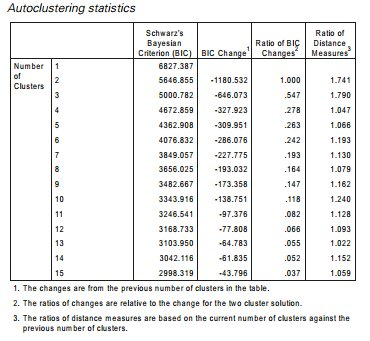
\includegraphics[width=10cm]{TwoStep1.jpg}\\
		\caption{Schwarz Bayesian Information Criterion}
	\end{centering}
\end{figure}


\end{document}